% MA211 - Lecture 04
\documentclass[pdftex, xcolor=pdftex, dvipsnames, handout]{beamer}

\usetheme{MA211}
\usepackage{thumbpdf}
\usepackage{wasysym}
%\usepackage{ucs}
\usepackage[utf8]{inputenc}
\usepackage{pgf,pgfarrows,pgfnodes,pgfautomata,pgfheaps,pgfshade}
\usepackage{verbatim}

\usepackage{eurosym}
\usepackage{euler}

\usepackage{calc}               % Simple computations with LaTeX variables
%\usepackage[hang]{caption2}     % Improved captions

\usepackage{graphicx}           % Standard graphics package

\usepackage{amsmath, amsthm, amssymb}


\newcommand{\fquad}{\mbox{\qquad}}
\newcommand{\bull}{$\bullet$ }

\newcommand {\I} {\mathcal I}
\newcommand {\calI} {\mathcal I}
\def\disint{\displaystyle\int}

\DeclareMathOperator{\D}{d}
\newcommand{\dydx}{\frac{\D y}{\D x}}

%\definecolor{gray}{rgb}{0.69, 0.69, 0.69} \newcommand{\gray}[1]{\textcolor{gray}{#1}}
\definecolor{dogreen}{rgb}{0.33, 0.42, 0.18} \newcommand{\dogreen}[1]{\textcolor{dogreen}{#1}}
\definecolor{maroon}{rgb}{.5,0.2,0.2}\newcommand{\maroon}[1]{\textcolor{maroon}{#1}}
\definecolor{greena}{rgb}{.1,0.581,0.1}\newcommand{\greena}[1]{\textcolor{greena}{#1}}

\definecolor{blue4}{rgb}{0,0,.545}
\newcommand{\Blue}[1]{\textcolor{blue}{#1}}
\newcommand{\Red}[1]{\textcolor{red}{#1}}
\definecolor{pink}{rgb}{1.,0.75,0.8}
\definecolor{darkred}{rgb}{0.5,0.0,0.0}
\definecolor{darkgreen}{rgb}{0,0.3,0.3}
\definecolor{purple}{rgb}{0,0.3,0.3}
\definecolor{darkblue}{rgb}{0.0, 0.0, .5}
\definecolor{dpurple}{rgb}{.3,.0,.3}
\newcommand{\Green}[1]{\textcolor{darkgreen}{#1}}
\newcommand{\DRed}[1]{\textcolor{darkred}{#1}}
\newcommand{\DBlue}[1]{\textcolor{darkblue}{#1}}
\newcommand{\Purple}[1]{\textcolor{dpurple}{#1}}
\newcommand{\Emph}[1]{\textcolor{darkred}{\textbf{\it #1}}}
\newcommand{\remph}[1]{\textcolor{darkred}{\textbf{\emph{#1}}}}
\newcommand{\bemph}[1]{\textcolor{darkblue}{\textbf{\emph{#1}}}}
\newcommand{\gemph}[1]{\textcolor{darkgreen}{\textbf{\emph{#1}}}}
\newcommand{\Bf}[1]{\textcolor{darkblue}{\textbf{#1}}}
\newcommand{\Gf}[1]{\textcolor{darkgreen}{\textbf{#1}}}
\newcommand{\Rf}[1]{\textcolor{red}{\textbf{#1}}}
\newcommand{\Rmf}[1]{\textcolor{red}{\mathbf{#1}}}

\newcommand{\Conj}[1]{\overline{#1}}

\newcommand{\code}[1]{\textcolor{darkblue}{\texttt{\textbf{#1}}}}
\newcommand{\icode}[1]{{\blue\texttt{\textbf{\emph{#1}}}}}
\newcommand{\gcode}[1]{{\Green{\texttt{\textbf{\emph{#1}}}}}}
\newcommand{\out}[1]{\texttt{\emph{\textbf{\Green{#1}}}}}





\newenvironment{vminipage}%
{\begin{Sbox}\begin{minipage}\begin{small}\begin{verbatim}}%
{\end{verbatim}\end{small}\end{minipage}\end{Sbox}\fbox{\TheSbox}}

\newenvironment{nminipage}%
{\begin{Sbox}\begin{minipage}}%
{\end{minipage}\end{Sbox}\fbox{\TheSbox}}


\let\Arg\relax\DeclareMathOperator{\Arg}{\mathtt{Arg}}
\let\Arg\relax\DeclareMathOperator{\e}{\mathtt{e}}

\newcommand {\AND} {\wedge}
\newcommand {\OR} {\vee}
\newcommand {\NOT} {\neg}
\newcommand {\IMPLIES} {\rightarrow}
%\newcommand {\IFF} {\leftrightarrow}
\renewcommand {\iff} {\Leftrightarrow}
\newcommand {\NAND} {\uparrow}
\newcommand {\NOR} {\downarrow}
\newcommand {\XOR} {\otimes}

\newenvironment{citemize}% Colour items
{\begin{description}}%
{\end{description}}

\newcommand {\maroonitem}{\item[\maroon{$\bullet$}]}

\newcommand {\gitem} {\item {\includegraphics[width=.4cm,angle=-10]{img/green-bullet-on-white.ps}}}
\newcommand {\ritem} {\item {\includegraphics[width=.4cm,angle=-10]{img/red-bullet-on-white.ps}}}
\newcommand {\yitem} {\item {\includegraphics[width=.4cm,angle=-10]{img/yellow-bullet-on-white.ps}}}
\newcommand {\bitem} {\item {\includegraphics[width=.4cm,angle=-10]{img/blue-bullet-on-white.ps}}}

\newcommand {\greenitem} {\item {\includegraphics[width=.4cm,angle=-10]{img/green-bullet-on-white.ps}}}
\newcommand {\reditem} {\item {\includegraphics[width=.4cm,angle=-10]{img/red-bullet-on-white.ps}}}
\newcommand {\yellowitem} {\item {\includegraphics[width=.4cm,angle=-10]{img/yellow-bullet-on-white.ps}}}
\newcommand {\blueitem} {\item {\includegraphics[width=.4cm,angle=-10]{img/blue-bullet-on-white.ps}}}

\newcommand {\eq}[1]%
  {$\DBlue{#1}$}
\newcommand {\eqd}[1]%
  {$\displaystyle\DBlue{#1}$}
%\newcommand{\eq}[1]{\boldmath \DBlue{$#1$}}


\newcommand {\csf}{\centerslidesfalse}
\newcommand {\cst}{\centerslidestrue}

\newcommand {\vecii}[2] {   \big(\begin{smallmatrix} #1 \\ #2 \end{smallmatrix}\big)}
\newcommand{\atwo}[2]{\left(\!\!\begin{array}{c} #1 \\ #2 \end{array}\!\!\right)}


\newcommand{\C}{\mathbb{C}}
\newcommand{\Q}{\mathbb{Q}}
\newcommand{\R}{\mathbb{R}}
\newcommand{\N}{\mathbb{N}}
\newcommand{\Z}{\protect\mathbb{Z}}  % protect for index.
\newcommand {\Rs}{ \mathbb{R}}
\newcommand {\Cs}{ \mathbb{C}}
\newcommand {\Rnn}{ \mathbb{R}^{n \times n}}
\newcommand {\Rn}{ \mathbb{R}^{n}}


\newcommand{\mblock}{%
\setbeamercolor*{block title}{bg=maroon,fg=white}
\setbeamercolor*{block body}{bg=white,fg=maroon}
}%

\newcommand{\bblock}{%
\setbeamercolor*{block title}{bg=Steel,fg=white}
\setbeamercolor*{block body}{bg=Mylightgray,fg=Steel}
}%

\newcommand{\gblock}{%
\setbeamercolor*{block title}{bg=Green,fg=white}
\setbeamercolor*{block body}{bg=Mylightgray,fg=darkgreen}
}%


\newcommand{\rblock}{%
\setbeamercolor*{block title}{bg=Red,fg=white}
\setbeamercolor*{block body}{bg=white,fg=Black}
}%


\newcommand{\TakeNotes}{
\includegraphics[width=2cm]{TakeNote}}

%\newcommand{\gblock}{%
%\setbeamercolor*{block title}{bg=Green,fg=white}
%\setbeamercolor*{block body}{bg=Mylightgray,fg=Green}
%}%


\def\eps{\varepsilon}
\newcommand {\del}[2]{ {\frac{\partial #1}{\partial #2}}}
\newcommand {\x}[1]{x^{[#1]}}
\newcommand {\delx}{ {\frac{\partial}{\partial x}}}
\newcommand {\delt}{ {\frac{\partial}{\partial t}}}
\newcommand {\dely}{ {\frac{\partial}{\partial y}}}
\newcommand {\ith}{{(i)}}
\renewcommand {\vec}[1]{ {\boldsymbol{#1}}}
\newcommand {\Oh} {\mathcal O}
\newcommand {\Err} {\mathcal E}
%\newcommand {\th} {\mathrm{th}}
\DeclareMathOperator{\fl}{fl}
\DeclareMathOperator{\sign}{sign}
\DeclareMathOperator{\Cond}{Cond} 
\DeclareMathOperator{\cond}{cond}
\DeclareMathOperator{\diag}{diag} 
\DeclareMathOperator{\sym}{sym} 
\DeclareMathOperator{\Trace}{Trace}
\DeclareMathOperator{\E}{e}

\newcommand {\Rsym}{{ \mathbb{R}^{n \times n}_\mathrm{sym}}}

\parskip .25cm


\theoremstyle{definition}
\newtheorem{exercise}{Exercise}[section]
\newtheorem{method}{Method}[section]



\subtitle{MA211}
\title{Lecture 4: Limits and Derivatives}

\author{Dr Niall Madden}

\date{\Large Wednesday 17 September 2008}


\begin{document}


\frame{

\begin{block}{}
\begin{center}
{\large \insertsubtitle}

\vspace{.1cm}

\begin{Large}
\textbf{\inserttitle}
\end{Large}

\vspace{.15cm}

% {\footnotesize \insertauthor}

\vspace{.3cm}

{ {\insertdate}}
\end{center}
\end{block}


\vspace{-0.25cm}
\begin{center}
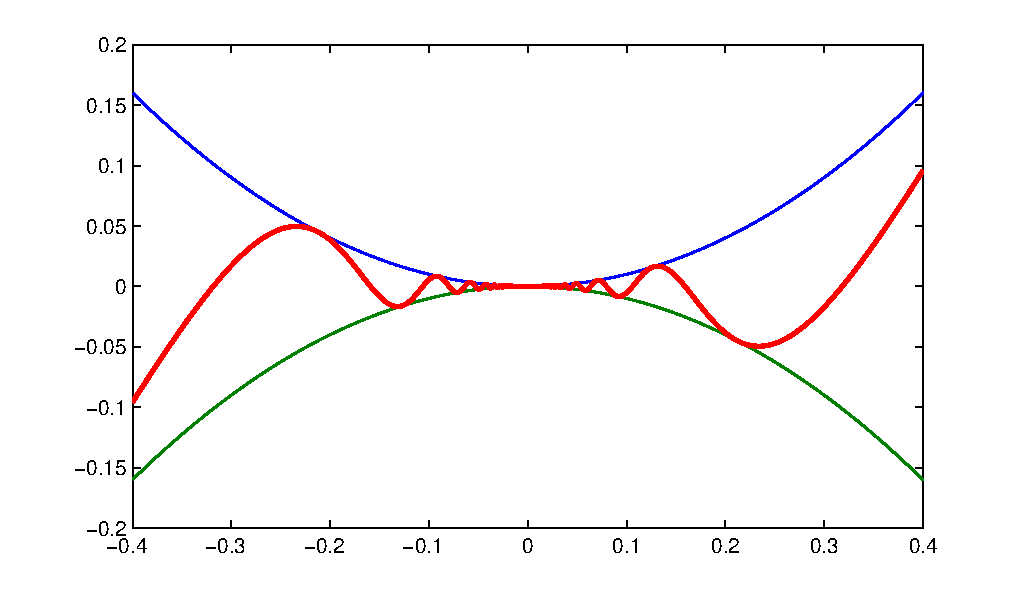
\includegraphics[height=4.5cm]{images/Squeeze}
\end{center}
}



%\section{Outline}
\frame{
  \frametitle{Outline}
 \tableofcontents



}


\frame{

\begin{center}
{\Large \Bf{Problem Solving Sessions}}
\end{center}

Reminder: Problem Solving Sessions (tutorials) will start next week. There will
be \Bf{two} per week. Attend whichever one you like
\begin{itemize}

\item Tuesday, 3pm, AC202

\item Wednesday, 5pm, QA003 (Physiology lecture room)


\end{itemize}

}

\section{Recall... Limits}
\frame{

When we write 
\[
\lim_{x \rightarrow c} f(x) = L
\]
or say ``\Emph{The limit of \eq{f} as \eq{x} approaches \eq{c} is
  \eq{L}}'' we mean that we can make \eq{f} as close to \eq{L} as we
  would like by taking \eq{x} as close to \eq{c} as is needed.

\pause

\begin{definition}[Limit]
If for any \eq{\eps>0}, no matter how small, we can find \eq{\delta>0}
such that
\[
|f(x) -L | < \eps ~~ \text{ when  } ~~ |x-c| < \delta.
\]
then we can say
\[
\lim_{x \rightarrow c} f(x) = L.
\]
\end{definition}
}

\frame{


As the end of \Emph{Lecture 3} we introduced problems of the following
form:
\begin{block}{}
\[
  \lim_{x \rightarrow c} \frac{f(x)}{g(x)} = 
\frac{\lim_{x \rightarrow c} f(x)}{\lim_{x \rightarrow c} g(x)}
\pause \quad \text{ where  } \quad \lim_{x \rightarrow c} g(x)
  = 0
\]
\end{block}
We'll look at two techniques for solving such problems:
\begin{itemize}
\item The  \Emph{The Squeeze Theorem} (\alert{today}).
\item \Emph{l'Hospital's Rule}
\end{itemize}

}

\subsection{The Squeeze Theorem}

\frame{

\begin{theorem}[The Squeeze Theorem]
Let \eq{f}, \eq{g} and \eq{h} be functions such that 
\[
f(x) \leq g(x) \leq h(x) \quad \text{ for } x \text { near } c.
\]
If
\[ 
\lim_{x \rightarrow c} f(x) = L \quad \text{ and } 
\lim_{x \rightarrow c} h(x) = L,
\]
then 
\[ \lim_{x \rightarrow c} g(x) = L.
\]
\end{theorem}

}

\frame{
\begin{example}
Show that 
\eqd{ \lim_{x  \rightarrow 0} x^2 \sin\big(\frac{1}{x}\big) = 0.}
\end{example}

\vspace{4cm}


}

%\frame{
%\begin{example}
%Use the Squeeze Theorem to show that
%\[
%\lim_{t \rightarrow 0} \frac{\sin(t)}{t} = 1.
%\]
%\end{example}
%
%\vspace{4cm}
%
%}



\frame{

\begin{exercise}[4.1]

Use the Squeeze theorem to answer the following questions.
\begin{enumerate}[(i)]
\item Find  \eq{\lim_{x \rightarrow 0} f(x)} if  $f$ is a function such that 
\[ 2-x^2 \leq f(x) \leq 2\cos(x),\]


\item If $\lim_{x \rightarrow 0} |f(x)|=0$, show that  $\lim_{x \rightarrow
    0} f(x)=0$.

\item What is the largest possible domain of  $f(x)=x^4\cos(2/x)$?

Show that  \eq{\lim_{x\rightarrow 0} f(x)=0}.


\end{enumerate}

\end{exercise}
}

\subsection{l'Hospital's Rule}
\frame{
The rule of l'Hospital is


\begin{block}{}
\[
\frac{\lim_{x \rightarrow c}  f(x)}{\lim_{x \rightarrow c}  g(x)} = 
\frac{\lim_{x \rightarrow c} f'(x)}{\lim_{x \rightarrow c} g'(x)}
\]
\end{block}
where here, for example,  \eq{f'(x)} is the \alert{derivative} of \eq{f} with
respect to \eq{x}.

And explaining what that means is one of the real reasons we've
introduced the idea of a limit.

We'll return to l'Hospital's rule toward the end of next Monday's
lecture.

}

\section{Derivatives}
\frame{
How can you calculate the slope of the tangent to a function \eq{f} at a
given point \eq{x}?

One approach is to compute the slope of the line that intersects 
the function at \eq{x} and some near by point \eq{x+h}. (This is
called a  \Emph{secant} line)...

And then get the limit of the slope of the secant lines as \eq{h}
tends to zero.

This gives us the definition
\begin{block}{}
\[
f'(x) :=  \frac{d}{dx}f(x) := \lim_{h \rightarrow 0} \frac{ f(x+h) -
  f(x)}{h}.
\]
\end{block}

}

\frame{
\begin{example}
Find the derivative of $f(x)=x^2$ using the above definition. (i.e,
``\emph{differentiate \eq{f(x)=x^2} from first principles}.'').
\end{example}

\vspace{4cm}
}

\frame{
\begin{example}
Find the derivative of $f(x)=1/x$ from first principles.
\end{example}
\vspace{4cm}

}




\frame{

\begin{exercise}[4.2]
From first principles, find the derivative of 
\begin{enumerate}[(a)]
\item \eqd{f(x)= \frac{1}{3} x^3.}
\item \eqd{f(x)= x^n} for any $n=1, 2, 3, ...$
\item \eqd{f(x)=  x^{-n}}

\end{enumerate}
\end{exercise}

For a hint for Part (ii), use the \Emph{binomial theorem} (see Slides
19 and 20).
}





\frame{
In the majority of cases, you don't have to use first principles to
calculate derivatives. The answer for the most common functions are
given in the \Emph{Mathematical (``Log'') Tables}.

We then use these, often in conjunction with some so-called rules, such
as the \Emph{Product Rule} and \Emph{Quotient Rule}, which are also
given in the tables. 

\pause 

\Bf{Elementary properties}
\begin{itemize}
\item \eq{\big(f+g\big)'(x)  = f'(x) + g'(x).}
\item \eq{\big(f-g\big)'(x)  = f'(x) - g'(x).}
\item \eq{\big(C f\big)'(x)  = Cf'(x)}, for a constant \eq{C}.
  \end{itemize}
}



\subsection{ $\big(u \cdot v\big)'(x)$}
\frame{

\begin{block}{The derivative of the product of 2 functions}
Let \eq{f(x) = u(x)v(x)}. Then
\[
\frac{d}{dx}f(x) = ( u\cdot v)'(x)  = u(x) v'(x)  +  u'(x) v(x).
\]
\end{block}

\vspace{3cm}

}


\frame{


\begin{example}
What is the derivative of 
\[
f(t) = (t^2 +1)(t^3 +2t)?
\]
\end{example}
\vspace{3cm}
}

\section{ $\big(u / v \big)'(t)$}
\frame{

\begin{block}{The derivative of the ratio of 2 functions}
Let \eq{f(x) = u(x)/v(x)}. Then
\[
f'(x)
=
\frac{v(x) u'(x)  -  u(x) v'(x)}{ \big(v(x)\big)^2}.
\]
\end{block}

We'll postpone a proof of this for a while.

}

\frame{

\begin{example}
Calculate the derivative of 
\[
f(t) =  \frac{\sqrt{t}}{2t -1}
\]
\end{example}

\vspace{3cm}

}


\section{Extra: Binomial Expansions}

\frame{

Exercise 4.2 (b) required us to find the derivative (with respect to
\eq{x}) of $f(x)=x^n$ for any $n=1, 2, 3, \dots$

This  involves working with the expression
\[
\lim_{h \rightarrow 0} \frac{(x+h)^n - x^n}{h}.
\]
So we need to expand the expression \eqd{(x+h)^n}, using the
\emph{Binomial Theorem}

}

\frame{

 Recall \Emph{Binomial Expansion}
\[ 
 (a  +  b)^n  =  a^n + \binom{n}{1}a^{n-1}b
+ \binom{n}{2}a^{n-2}b^2 + \cdots + \binom{n}{n-1}ab^{n-1} + b^n
\]
\pause
\[ 
 (a  +  b)^n  =
\sum_{k=0}^n
  \binom{n}{k}  a^{n-k}  b^k,
\]
Here  the  \Emph{Binomial  Coefficient}
  $\binom{n}{k}$   (``$n$  choose   $k$'')  is   
\[
  \binom{n}{k}  =  \frac{n!}{k!\,  (n-k)!},  
\]
and   $n!$  (``$n$  factorial'') is $n! = n \cdot (n-1) \dots 3 \cdot 2
\cdot 1$.

}


\end{document}
